\documentclass[12pt]{article}

% Paquetes solicitados
\usepackage[spanish]{babel}
\usepackage{amsmath}
\usepackage{graphicx}
\usepackage{float} % Permite usar [H] para fijar las imágenes exactamente en su lugar

\title{Recetario de Comida Mexicana}
\author{Jesús Emilio Jiménez Aguilar 286666}
\date{}

\begin{document}

\maketitle

\section{Introducción}
Este documento presenta un recetario de comida mexicana elaborado en \LaTeX{},
el cual incluye cinco recetas tradicionales utilizando lo aprendido en clase.

\section{Receta 1: Chilaquiles Rojos}

\subsection{Ingredientes}
\begin{itemize}
    \item Totopos
    \item Jitomate
    \item Chile guajillo
    \item Cebolla
    \item Ajo
    \item Crema
    \item Queso fresco
\end{itemize}

\subsection{Procedimiento}
Licúa el jitomate con el chile, ajo y cebolla.
Fríe la salsa y agrega los totopos.
Sirve con crema y queso.

\begin{figure}[H]
    \centering
    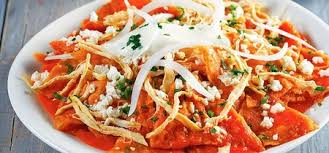
\includegraphics[width=0.5\textwidth]{chilaquiles (1).jpg}
    \caption{Chilaquiles rojos}
\end{figure}

\section{Receta 2: Bistec a la Mexicana}

\subsection{Ingredientes}
\begin{itemize}
    \item Bistec de res
    \item Jitomate
    \item Cebolla
    \item Chile serrano
    \item Aceite
    \item Sal
\end{itemize}

\subsection{Procedimiento}
Fríe la carne, agrega jitomate, cebolla y chile.

\begin{figure}[H]
    \centering
    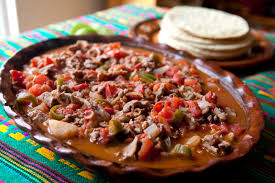
\includegraphics[width=0.5\textwidth]{bistec (1).jpg}
    \caption{Bistec a la mexicana}
\end{figure}

\section{Receta 3: Revoltillo Verde}

\subsection{Ingredientes}
\begin{itemize}
    \item Huevos
    \item Salsa verde
    \item Aceite
    \item Sal
\end{itemize}

\subsection{Procedimiento}
Calienta el aceite en una sartén, vierte la salsa verde y agrega los huevos batidos.
Cocina revolviendo.

\begin{figure}[H]
    \centering
    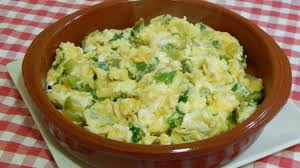
\includegraphics[width=0.5\textwidth]{revoltillo (1).jpg}
    \caption{Revoltillo verde}
\end{figure}

\section{Receta 4: Huevos Divorciados}

\subsection{Ingredientes}
\begin{itemize}
    \item Huevos
    \item Tortillas
    \item Salsa roja
    \item Salsa verde
    \item Frijoles refritos
\end{itemize}

\subsection{Procedimiento}
Fríe las tortillas y los huevos.
Sirve un huevo con salsa roja y otro con salsa verde,
acompañados de frijoles.

\begin{figure}[H]
    \centering
    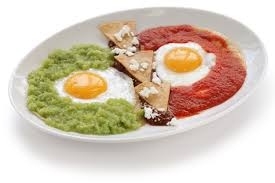
\includegraphics[width=0.5\textwidth]{huevos_divorciados (1).jpg}
    \caption{Huevos divorciados}
\end{figure}

\section{Receta 5: Tacos al Pastor}

\subsection{Ingredientes}
\begin{itemize}
    \item Carne de cerdo
    \item Achiote
    \item Piña
    \item Tortillas
    \item Cebolla
    \item Cilantro
\end{itemize}

\subsection{Procedimiento}
Marina la carne con achiote.
Cocina y sirve en tortillas con piña,
cebolla y cilantro.

\begin{figure}[H]
    \centering
    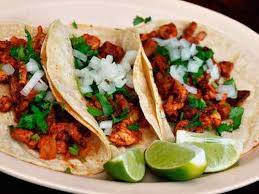
\includegraphics[width=0.5\textwidth]{tacos_pastor (1).jpg}
    \caption{Tacos al pastor}
\end{figure}

\section{Conclusión}
La gastronomía mexicana es rica en variedad y sabor. El uso de herramientas como \LaTeX{} permite documentar estas tradiciones de manera formal y estructurada.

\end{document}
\begin{figure}
    \centering
    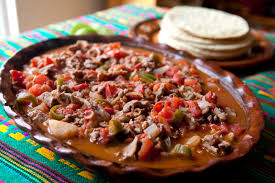
\includegraphics[width=0.5\linewidth]{bistec (1).jpg}
    \caption{Enter Caption}
\begin{figure}
        \centering
        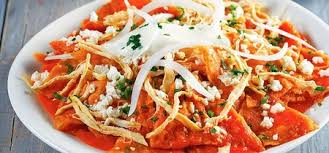
\includegraphics[width=0.5\linewidth]{chilaquiles (1).jpg}
        \caption{Enter Caption}
\begin{figure}
            \centering
            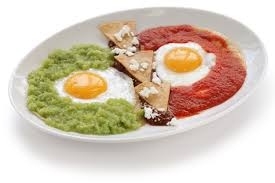
\includegraphics[width=0.5\linewidth]{huevos_divorciados (1).jpg}
            \caption{Enter Caption}
\begin{figure}
                \centering
                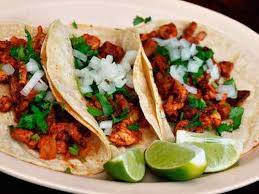
\includegraphics[width=0.5\linewidth]{tacos_pastor (1).jpg}
                \caption{Enter Caption}
\begin{figure}
                    \centering
                    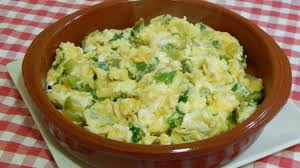
\includegraphics[width=0.5\linewidth]{revoltillo (1).jpg}
                    \caption{Enter Caption}
                    \label{fig:placeholder}
                \end{figure}
                                \label{fig:placeholder}
            \end{figure}
                        \label{fig:placeholder}
        \end{figure}
                \label{fig:placeholder}
    \end{figure}
        \label{fig:placeholder}
\end{figure}